% XCircuit output "proteccion.tex" for LaTeX input from proteccion.eps
\def\putbox#1#2#3#4{\makebox[0in][l]{\makebox[#1][l]{}\raisebox{\baselineskip}[0in][0in]{\raisebox{#2}[0in][0in]{\scalebox{#3}{#4}}}}}
\def\rightbox#1{\makebox[0in][r]{#1}}
\def\centbox#1{\makebox[0in]{#1}}
\def\topbox#1{\raisebox{-0.60\baselineskip}[0in][0in]{#1}}
\def\midbox#1{\raisebox{-0.20\baselineskip}[0in][0in]{#1}}
   \scalebox{1}{
   \normalsize
   \parbox{4.66667in}{
   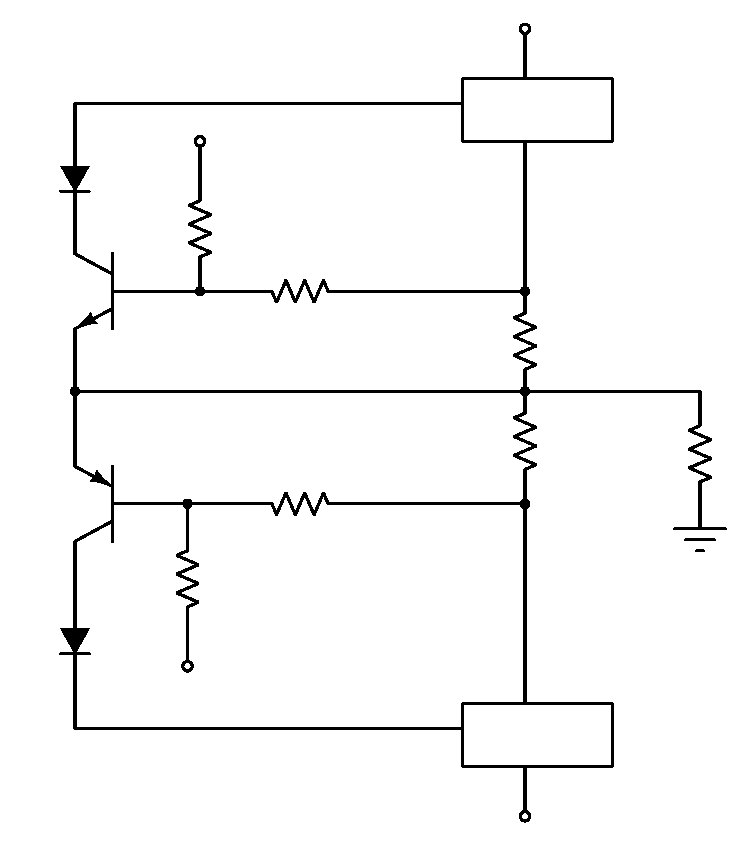
\includegraphics[scale=1]{proteccion}\\
   % translate x=3040 y=-1322 scale 0.38
   \putbox{3.14in}{4.84in}{1.20}{Etapa}%
   \putbox{3.06in}{4.67in}{1.20}{de salida}%
   \putbox{3.14in}{0.67in}{1.20}{Etapa}%
   \putbox{3.06in}{0.50in}{1.20}{de salida}%
   \putbox{4.14in}{2.42in}{1.20}{RL}%
   \putbox{3.64in}{3.50in}{1.20}{Re}%
   \putbox{3.56in}{2.50in}{1.20}{Re}%
   \putbox{0.72in}{4.00in}{1.20}{R60}%
   \putbox{1.72in}{3.75in}{1.20}{R59}%
   \putbox{1.72in}{2.34in}{1.20}{R57}%
   \putbox{1.31in}{1.67in}{1.20}{R58}%
   \putbox{0.06in}{3.50in}{1.20}{Q52}%
   \putbox{0.06in}{2.09in}{1.20}{Q53}%
   \putbox{1.39in}{4.00in}{1.20}{22k}%
   \putbox{1.72in}{3.34in}{1.20}{270}%
   \putbox{1.72in}{1.92in}{1.20}{270}%
   \putbox{0.72in}{1.59in}{1.20}{22k}%
   } % close 'parbox'
   } % close 'scalebox'
   \vspace{-\baselineskip} % this is not necessary, but looks better
